% =========================================================
% TikZ diagram: Unit balls under different p-norms
% Place after metric definition or examples section.
% Requires: \usepackage{tikz}
%           \usepackage{amsmath, amssymb}
%           \usepackage{caption}   (for \captionof)
% =========================================================

\begin{center}
\small\textbf{Unit balls $B_1(0)$ under $\ell^p$ metrics on $\mathbb{R}^2$}

\medskip
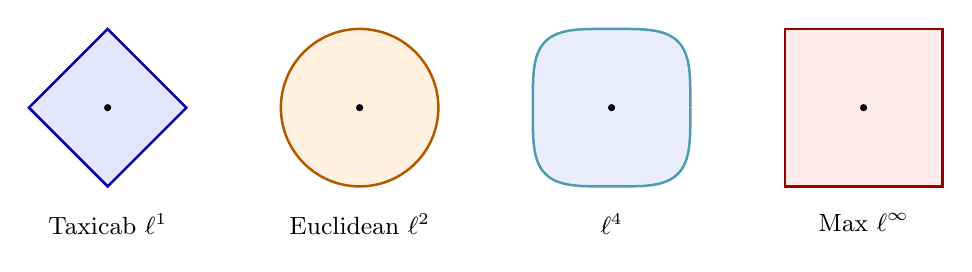
\begin{tikzpicture}[scale=1.0, line width=0.9pt]
\def\dx{3.2}
\def\s{1}
% L1
\begin{scope}[shift={(0,0)}]
  \fill[blue!10] (0,\s) -- (\s,0) -- (0,-\s) -- (-\s,0) -- cycle;
  \draw[blue!65!black] (0,\s) -- (\s,0) -- (0,-\s) -- (-\s,0) -- cycle;
  \fill (0,0) circle (1.3pt);
  \node[below=6pt, font=\small] at (0,-\s) {Taxicab $\ell^1$};
\end{scope}
% L2
\begin{scope}[shift={(\dx,0)}]
  \fill[orange!12] (0,0) circle (\s);
  \draw[orange!70!black] (0,0) circle (\s);
  \fill (0,0) circle (1.3pt);
  \node[below=6pt, font=\small] at (0,-\s) {Euclidean $\ell^2$};
\end{scope}
% L4
\begin{scope}[shift={(2*\dx,0)}]
  \fill[green!10!blue!8, line width=0pt]
    plot[domain=0:360,samples=200,smooth]
    ({\s*sign(cos(\x))*abs(cos(\x))^(1/2)},
     {\s*sign(sin(\x))*abs(sin(\x))^(1/2)}) -- cycle;
  \draw[green!45!blue!70]
    plot[domain=0:360,samples=200,smooth]
    ({\s*sign(cos(\x))*abs(cos(\x))^(1/2)},
     {\s*sign(sin(\x))*abs(sin(\x))^(1/2)});
  \fill (0,0) circle (1.3pt);
  \node[below=6pt, font=\small] at (0,-\s) {$\ell^4$};
\end{scope}
% L∞
\begin{scope}[shift={(3*\dx,0)}]
  \fill[red!8] (-\s,-\s) rectangle (\s,\s);
  \draw[red!60!black] (-\s,-\s) rectangle (\s,\s);
  \fill (0,0) circle (1.3pt);
  \node[below=6pt, font=\small] at (0,-\s) {Max $\ell^\infty$};
\end{scope}
\end{tikzpicture}

\smallskip
\begin{tabular}{cl}
  $\ell^1$:      & $d(x,y) = |x_1-y_1| + |x_2-y_2|$ \\[3pt]
  $\ell^2$:      & $d(x,y) = \sqrt{(x_1-y_1)^2 + (x_2-y_2)^2}$ \\[3pt]
  $\ell^4$:      & $d(x,y) = \bigl(|x_1-y_1|^4 + |x_2-y_2|^4\bigr)^{1/4}$ \\[3pt]
  $\ell^\infty$: & $d(x,y) = \max\bigl(|x_1-y_1|,\,|x_2-y_2|\bigr)$ \\
\end{tabular}

\smallskip
\captionof{figure}{Unit balls $\{\,y \in \mathbb{R}^2 : d(0,y) \le 1\,\}$
under four $\ell^p$ metrics on $\mathbb{R}^2$.
As $p$ increases from $1$ to $\infty$, the unit ball transitions from a
diamond ($\ell^1$) through the familiar disc ($\ell^2$) to a square
($\ell^\infty$).
All four metrics are strongly equivalent: there exist $c, C > 0$ such
that $c\,d_2(x,y) \le d_p(x,y) \le C\,d_2(x,y)$ for all $x,y \in \mathbb{R}^2$,
so they induce the same topology.}
\label{fig:unit-balls}
\end{center}